% !TEX root =../thesis-letomes.tex

\chapter{Search Strategies}
\section{Evolution Strategies}
We are basing our machine learning efforts on the Evolution Strategy (ES) algorithm outlined by Salimans et al. \cite{Salimans2017} using ES--it being a gradient estimator--makes sense in optimization scenarios where calculating an exact gradient is expensive. The idea is to sample around a starting point, and use a weighted average fitness score to pick a direction to move each cycle. It is generally applicable to unsupervised problems, such as ours; a reinforcement learning problem. There are several flavors of the concept under the ES umbrella term: Covariance Matrix Adaptation (CMA-ES), Natural Evolution Strategy (NES), and Exponential NES, to name a few. The one used in \cite{Salimans2017} and by extension in our project is NES. Its exact implementation details will follow:


\subsection{Theoretical Advantages and Disadvantages of ES Compared to RL}

\subsection{NES Algorithm}
In formal terms: Let \(F\) be the objective function with parameters \(\theta\). NES is the population from a distribution over parameters \(p_\psi (\theta)\), with hyperparameters \(\psi\). The procedure is then to optimize the expected objective value \(E_{\theta \sim p_\psi} F(\theta)\) by searching for \(\psi\) with stochastic gradient ascent. The gradient steps are taken with the estimator: \cite{Salimans2017}.
\begin{equation}
    \nabla_\psi E_{\theta \sim p_\psi} F(\theta)
    = E_{\theta \sim p_\psi} \{F(\theta)~\nabla_\psi~log~p_\psi(\theta)\}
\end{equation}
In our problem, \(F\) is the stochastic score returned by our environment (the Earth-Mars-Sun system) with \(\theta\) representing the policy of an agent in the environment ($\Delta v$ for our spacecraft's path) and \(\psi\) being the parametrization of that policy (launch parameters: angle, velocity, launch-time). The algorithm mutates the launch parameters \(\psi\), checks how the resulting path \(\theta\) performs in the environment \(F\) and moves around the resulting n-dimensional optimization space with gradient descent along its estimated gradient, defined by a normally distributed weighted point cloud \(\epsilon\).

\begin{figure}
    \centering
    \subfloat[Starting at some random point, the first iteration computes the fitness of a surrounding point cloud ($\epsilon$), and takes a step of size $\alpha$ in the direction of the weighted mean of $\epsilon$.]{
        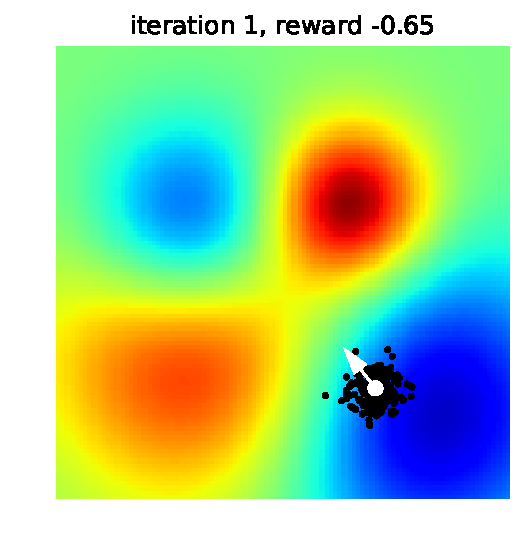
\includegraphics[width=0.46\linewidth]{fig/ES_basic_0}
        \label{fig:esbasic0}
    }
    \hfill
    \subfloat[this process continues each iteration, until we find ourselves at a local maximum (this example version is doing gradient \textit{ascent})]{
        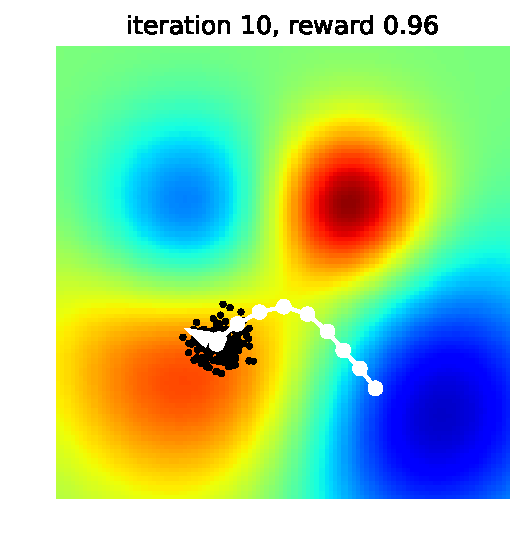
\includegraphics[width=0.46\linewidth]{fig/ES_basic_9}
        \label{fig:esbasic9}
    }
    \caption{the fundamental ES algorithm illustrated in a toy problem. Generated from code based on \cite{Salimans2017}}
    \label{fig:esbasic}

\end{figure}



\section{Brute Force "Fan Search"}
In \cite{Saxe2015}, the search strategy was significantly simpler than here, and it serves as the point of comparison for our search efforts. The way it was done is that the same three parameters contained in $\psi$ were tested in a three-dimensional fan arrangement. For example, the starting position $\psi_{pos}$ was defined from 0 to $2\pi$, the burn angle $\psi_{ang}$ was defined between 0 and $-\frac{\pi}{4}$, and the burn vector's magnitude $\psi_{burn}$ was defined between 3 and 3.8. The search strategy was then to evaluate the superposition of these three intervals, with e.g 100 values linearly spaced throughout each 'fan'. The set of values with the best score ($\psi\star$) would then be selected for refinement, where a smaller fan (tighter intervals) would be created, centered around $\psi\star$. The process would then repeat for some number of steps, constantly zeroing in on the best candidate.

For anyone with optimization experience it will be obvious that this method is very sensitive to local minimum issues. It doesn't anneal, or compute any kind of gradient, definite or estimated. It relies heavily on empirically defined starting parameters for determining the initial search intervals, so it's very specific to this problem. It is, in short, not really universal, or particularly intelligent, and was thus seen as an obvious candidate for improvement in this project.